%!TEX root = ../dokumentation.tex

\chapter{Datengenerierung}

\section{Random Sampling}

Mit Random Sampling ist eine Zufallsstichprobe gemeint bei der eine Stichprobe aus einer Grundgesamtheit $X$ mit $n$ Elementen gezogen wird. Seien die Elemente der Grundgesamheit $x_1,x_2,\dots,x_n-1,x_n$, dann unterliegt die Auswahl eines Elements $x \in M$ einem Auswahlverfahren, das angibt mit welcher Auftrittswahrscheinlichkeit $P(x)$ ein Element in die Stichprobe $N$ gelangen kann.
Es gelten die Bedingungen:
\begin{itemize}
    \item $P(x) > 0$ (Positivität)
    \item $\sum_{i=1}^{n}P(x_i)=1$ (Vollständigkeit)
\end{itemize}

Bei einer einfachen Zufallsstichprobe handelt es sich um die Auswahl einer Teilmenge einer statistischen Population, bei der jedes Element die gleiche Wahrscheinlichkeit $P(x)=\frac{1}{\lvert M \rvert}=\frac{1}{n}$ hat, ausgewählt zu werden. Zudem darf eine Ziehung aus einer Gesamtmenge nicht die nachfolgenden Ziehungen beeinflussen, weil sie unabhängig voneinander erfolgen müssen. Übertragen auf das typische Urnenexperiment der Stochastik, kommt es bei einer einfachen Zufallsstichprobe zu einer Ziehung mit Zurücklegen.

Für die Generation von Trainingsdaten ist das Random Sampling von großer Bedeutung, weil nur durch Einbeziehung einer Zufallskomponente neue Datensätze generiert werden können. Genau genommen handelt es sich bei der gewählten Vorgehensweise des Graph-Editors nur um eine Ziehung von einem einzigen Element. Der Grund hierfür liegt darin, dass nicht pro Feature in der $n$-zeiligen Ergebnismenge auch gleich $n$ Elemente auf einmal aus der Grundgesamtheit gezogen werden, sondern in jedem Durchgang wird ein Element mit einer bestimmten Wahrscheinlichkeit gezogen, welches dann zur weiteren Berechnungen von anderen Features einfließen kann. Die Knoten können sich so auf eine einelementige Ziehung beschränken, welche dann beliebig oft ausgeführt weden kann, je nachdem wie viele Datensätze generiert werden sollen.

Sollen beispielsweise zufällig ortspezfische Personendaten generiert werden, könnte die Herausforderung bestehen Daten von hunderten Personen aus nur vier Wohnorten zu generieren. Jeder Person soll dabei ein Wohnort zugewiesen werden, der zufällig bestimmt wird. Ist die Wahrscheinlichkeit für die Auswahl eines Wohnorts gleich groß, so ergibt sich eine einfache Zufallsstichprobe. Oft genügt eine Gleichverteilung jedoch nicht, um eine Zufallsvariable zu modellieren, weil in der Realität andere Faktoren die Wahrscheinlichkeitsverteilung beeinflussen. Will man bezogen auf die Generation von Personendaten beispielsweise Größen generieren, wird eine Normal-, auch Gauß- oder Glockenverteilung benötigt. Es kann auch sein, dass die Wahrscheinlichkeitsverteilung so spezifisch definiert ist, dass sie nicht mit einer einzigen Funktion dargestellt werden kann.

In den folgenden Kapiteln soll auf die genannten Fälle und deren Umsetzung eingegangen werden.

\subsection{Generation von gleichverteilten Zufallszahlen}

Für die einfache Zufallsstichprobe kann das Problem auf die Frage reduziert werden, wie eine gleichverteilte Zufallszahl in dem Intervall $I=[0;1]$ generiert werden kann. Diese Zufallszahl kann dann auf ein beliebiges Intervall transformiert werden. Sei $x_1$ eine gleichverteilte Zufallszahl im Intervall $I_1=[0;1]$ und seien $a$, $b$ Grenzen des Intervalls $I_2=[a;b]$, so ist die Zufallszahl $x_2$ im intervall $I_2$ bestimmt durch $x_2=x_1 \cdot b+a$. Durch das Runden auf die Einerstelle, können so auch diskrete Werte resultieren.

Um gleichverteilte Zufallszahlen generieren zu können, wird ein \ac{PRNG} verwendet. Ein \ac{PRNG} oder auch Zufallszahlengenerator stellt einen Algorithmus dar, der eine Sequenz von Zufallszahlen generiert. Es handelt sich bei den generierten Zahlen um Pseudo-Zufallszahlen, weil das zugrundeliegende Verfahren deterministisch implementiert ist. Bei gleichen Eingangsparametern ist auch immer das gleiche Ergebnis zu erwarten. 

Der essentielle Parameter eines \ac{PRNG}s ist der sogenannte Seed. Der Seed ist ein Startwert, der bei dem allerersten Aufruf des \ac{PRNG}s initial gesetzt wird. Aufbauend auf diesem Seed können alle weiteren Zufallszahlen generiert werden. Jeder generierte Wert wird als neuer Startwert für das Verfahren verwendet. Da der mögliche Wertebereich durch eine festgelegte Speichergröße begrenzt ist, muss zwangsläufig irgendwann eine Zahl generiert werden, die bereits in der Sequenz aufgetaucht ist. Weil sich die generierte Sequenz wiederholt, ist der Zufallszahlengenerator periodisch. Simple lineare Kongruenzgeneratoren durchlaufen den Wertebereich im besten Fall einmal pro Periode, weil sie mit nur einem Seed als initialen Wert arbeiten. Andere \ac{PRNG}s wie zum Beispiel der Mersenne-Twister arbeiten mit mehreren Seeds, wodurch eine erheblich größere Periodenlänge erreicht werden kann.

Ein Algorithmus kann Pseudo-Zufallszahlen generieren, die sich nur in einer bestimmten Anwendung nicht von echten Zufallszahlen unterscheiden lassen. Manche Generatoren sind deshalb für bestimmte Anwendungen gut geeignet und andere wiederum nicht. Müssen beispielsweise lange Sequenzen von Zufallszahlen generiert werden, ist ein linearer Kongruenzgenerator nicht zu empfehlen. Hingegen wäre er bei einer performanten Generation von kurzen Sequenzen eher geeignet. Echte Zufallszahlen verhalten sich immer gleich und bieten hohe Güte. Zur Generation von echten Zufallszahlen kommen pyhsikalische Zufallszahlengeneratoren zum Einsatz, die die naturgemäße Zufälligkeit von physikalischen Prozessen zu Nütze machen. Beispiele für solche physikalischen Prozesse sind Spannungsschwankungen an einer Z-Diode, thermisches Rauschen eines Widerstands und radioaktive Zerfallsvorgänge. Logischerweise ist die Benutzung eines Seeds und damit die Reproduzierbarkeit von physikalischen Zufallszahlengeneratoren nicht gegeben.

Die Möglichkeit einen Seed verwenden zu können, hat allerdings den großen Vorteil der Reproduzierbarkeit von Ergebnissen, weshalb die Verwendung von echten Zufallszahlen für den \ac{MLTDG} unpassend ist. Gerade bei der Erstellung von komplexen Zusammenhängen innerhalb der Applikation soll ein Neustart der Generation nach kleinen Veränderungen nicht komplett neue Daten generieren. Dem Benuter soll es möglich sein benutzerdefinierte Zufallsvariablen mit einem Seed zu versehen, um gleiche Ausgangswerte erhalten zu können.

Vorteile von Seeds:
\begin{itemize}
    \item Portabilität: Durch Speicherung der Seed-Werte bei einem Projektexport, werden bei unverändertem Projekt immer gleiche Trainingsdaten generiert, sodass das Projekt geteilt und wiederverwendet werden kann. 
    \item Debugging: Werden unerwartete Trainingsdaten generiert, können mithilfe von Seeds einzelne Änderungen vorgenommen werden, sodass die neuen Daten mit den letzten abgeglichen werden können. Aufgedeckte Singularitäten können so aufgedeckt und reproduziert werden. 
\end{itemize}

Es gibt einige JavaScript-Bibiliotheken, die \ac{PRNG}s bereits implementieren. Die Auswahl der Bibiliothek ist auf Chance.js gefallen aus den folgenden Gründen:
\begin{itemize}
    \item Einfache Nutzung durch die Verfügbarkeit als NPM-Package
    \item Ausführliche Dokumentation
    \item Verwendung eines Seeds
    \item Hohe Qualität durch integrierte Unit-Tests
\end{itemize}

\subsection{Generation von nicht-gleichverteilten Zufallszahlen}

Oft unterliegen Zufallsvariablen keiner gleichverteilten, sondern einer anderen Wahrscheinlichkeitsverteilung wie zum Beispiel die Normalverteilunge oder Exponentialverteilung. In diesem Fall ein Verfahren benötigt, um aus einer gleichverteilten Zufallszahl eine Zufallszahl einer anderen Wahrscheinlichkeitsverteilung zu generieren.

Die Inversionsmethode ist ein Algorithmus, der bei mehrfachem Aufruf eine Sequenz von Zufallszahlen $x_0, x_1, x2$ generiert, die einem vorgegeben stochastischem Modell entspringen. Der Algorithmus beschäftigt sich mit dem Problem, eine beliebige Verteilung auf $\mathbb{R}$ abzubilden. Neben der Verteilungsfunktion ist eine Voraussetzung für die Inversionsmethode ein vorhandener Zufallszahlengenerator, der gleichverteilte Zufallszahlen im Intervall $I=[0,1]$ generieren kann \cite{Inversionsmethode}. Hierfür kann der \ac{PRNG} der Bibliothek Chart.js aus dem letzten Kapitel herangezogen werden.

Das Inversionsprinzip ist wie folgt definiert:\\
Es sei $F$ eine Verteilungsfunktion und $U$ eine $U(0,1)$-verteilte Zufallsvariable.\\
Dann gilt \cite{Inversionsmethode}: $Y = F^{-1}(U)$ hat die Verteilungsfunktion $F$, d. h.
$$P(Y \le t)=F(t),t \in \mathbb{R}$$

Das Hauptproblem ist damit die Bestimmung der Inversen einer Verteilungsfunktion. Da nicht jede Funktion umkehrbar ist, kann dieses Verfahren nur für bestimmte Wahrscheinlichkeitsfunktionen verwendet werden. Im Folgenden wird die Berechnung der Inversen für die im \ac{MLTDG} relevanten Verteilungen erläutert.

Die Exponentialverteilung ist eine stetige Wahrscheinlichkeitsverteilung über der Menge der positiven reellen Zahlen. Sie wird häufig verwendet, um die Dauer von Zeitintervallen zu modellieren:
\begin{itemize}
    \item Dauer eines Telefongesprächs
    \item Alter von Lebewesen
    \item Zeitspanne zwischen zwei Anrufen
    \item Lebensdauer von Geräten
\end{itemize}
Die Verteilungsfunktion der Exponentialverteilung 
$$F(X)=1-e^-\lambda x$$
berechnet die Auftrittswahrscheinlichkeit des nächsten Ereignisses im Intervall $[0;x]$.\\
Die Inverse ist definiert durch
$$x=F^-1(y)=-\frac{1}{\lambda}ln(1-y)$$

Die Inversionsmethode gelingt nicht immer, weil nicht jede Funktion auch umkehrbar ist. Nur für Funktionen von denen die Inverse gebildet werden kann, kann dieses Verfahren zur Erzeugung von Zufallszahlen mit der durch die Funktion beschriebenen Verteilung eingesetzt werden. Eine weitere wichtige Verteilung ist die Normalverteilung für die unmittelbar keine Inverse ermittelt werden kann. 

Die Normalverteilung ist eine stetige Wahrscheinlichkeitsverteilung mit großer Bedeutung, weil sich viele Prozesse natur-, wirtschafts- und ingenieurswissenfschaftlicher Herkunft entweder exakt oder näherungsweise mit ihr darstellen lassen.\\ 
Die Normalverteilung $\mathcal{N}(\mu,\sigma ^2)$ ist definiert durch die Parameter: 
\begin{itemize}
    \item $\mu$: Erwartungswert
    \item $\sigma$: Standardabweichung
\end{itemize}
Eine stetige Zufallsvariable X heißt normalverteilt, wenn die Wahrscheinlichkeit für $X \le x$ ist, sodass das Integral der Gaußschen Fehlerfunktion gegeben ist mit:
\medskip
$$P(X \le x)=\frac{1}{\sigma\sqrt{2\pi}}\int_{-\infty}^{x}e^{-\frac{1}{2}(\frac{t-\mu}{\sigma})^2}dt$$
\medskip
Deren erste Ableitung
\medskip
$$f(x)=\frac{1}{\sigma\sqrt{2\pi}}e^{-\frac{1}{2}(\frac{t-\mu}{\sigma})^2}$$
\medskip
ist die Dichtefunktion der Normalverteilung \cite{Inversionsmethode}.

Es gibt einige Methoden, um normalverteilte Zufallszahlen zu generieren, obwohl das Fehlerintegral nicht unmittelbar bestimmbar ist. Im Folgenden werden relevante Algorithmen zur Vollständigkeit aufgezählt aber auf sie nicht näher eingegangen. 
\begin{itemize}
    \item Ziggurat-Algorithmus
    \item Box-Muller-Methode
    \item Polar-Methode
\end{itemize}

\subsection{Generation von Zufallszahlen einer benutzerdefinierten Wahrscheinlichkeitsverteilung}

Steht man vor der Aufgabe Daten zu generieren, die von einer Zufallsvariable abhängen, deren Wahrscheinlichkeitsverteilung sehr komplex ist, ist es oft nur mit sehr großem Aufwand, wenn überhaupt, möglich eine Funktion zu finden. In diesem Fall soll der Benutzer in der Lage sein, schnell und einfach mit einer grafischen Oberfläche die gewünschte Wahrscheinlichkeitsverteilung zu modellieren. Dadurch wird zum einen eine konzeptuelle Umgebung geschaffen, als auch der Aufwand erspart eine exakte Dichtefunktion der Wahrscheinlichkeitsverteilung zu entwerfen. Selbst wenn es keine Dichtefunktion für die Wahrscheinlichkeitsverteilung gibt, könnte sie immernoch näherungsweise modelliert werden.

Die Gestaltung einer Oberfläche unterscheidet sich hierbei maßgeblich dabei, ob es sich um eine stetige oder diskrete Wahrscheinlichkeitsverteilung handelt. Ein Verteilungsdiagramm für stetige Werte wird mit einer Kurve modelliert. Hingegen wird ein Verteilungsdiagramm für kontinuierliche Werte ein Säulendiagramm verwendet. Die in BaklavaJS erstellen Nodes werden mit $CustomNode$ für kontinuierliche Werte und $DiscreteNode$ für diskrete Werte referenziert.

Die Vorgehensweise besteht aus den drei Komponenten: 
\begin{enumerate}
    \item Grafische Benutzeroberfläche (UI)
    \item Spline-Interpolation
    \item Erzeugung der Zufallszahl
\end{enumerate}
$CustomNode$ und $DiscreteNode$ unerscheiden sich hierbei lediglich bei der ersten Komponente, der grafischen Benutzeroberfläche. Die anderen zwei Komponenten decken sich bei beiden Nodes.

In den folgenden Kapitel wird auf die Umsetzung der einzelnen Komponenten eingegangen.

\subsubsection{Benutzerdefinierte Erstellung einer Wahrscheinlichkeitsverteilung}

Für die grafische Oberfäche der beiden Nodes wird ein freier Zeichenraum benötigt, auf dem das Linien- und Säulendiagramm gezeichnet werden kann. Zudem soll die Oberfläche Interaktionsmöglichkeiten zur Gestaltung der Verteilung geben. Hierbei fällt die Auswahl wie in Kapitel 2.2 auf die beiden Technologien SVG und Canvas. Da es bereits einige Implementierungen von Visualisierungsmöglichkeiten in JavaScript gibt, wird auch an dieser Stelle an eine bereits existierende Lösung zurückgegriffen. Hierfür wird das JavaScript Framework Chart.js verwendet aus den folgenden Gründen \cite{chartjs}:
\begin{itemize}
    \item Open-Source + MIT License: Freie Nutzung ohne anfallende Kosten
    \item Unterstützung von 8 Chart-Typen: Inklusive Linien- und Säulendiagramm
    \item HTML5 Canvas: Gute Rendering Performanz
    \item Responsive: Diagramme werden in einer skalierbaren Sidebar verwendet
\end{itemize}

Für die stetige Wahrscheinlichkeitsverteilung müssen in dem Liniendiagramm Interaktionsmöglichkeiten zum Hinzufügen (Doppelklick), Löschen (Rechtsklick) und Verschieben (Linkslick) von Punkten implementiert werden. Die Punkte sind mit einer Linie miteinander verbunden. Im linearen Modus werden zwei aufeinanderfolgende Punkte mit einer Geraden verbunden.

Das Säulendiagramm für die diskrete Wahrscheinlichkeitsverteilung soll dem Nutzer die Möglichkeit geben die einzelnen Säulenhöhen zu setzen (Linksklick). Ein wichtiges Detail ist bei dem Setzen der Säulenhöhen, dass dies auch funktionieren soll, wenn der Zeiger sich bei gehaltener Taste über mehrere Säulen bewegt, weil die Gestaltung des Verteilungsdiagramms sonst bei einem großen Wertebereich sehr aufwändig wird. 

\begin{figure}[H]
    \center
    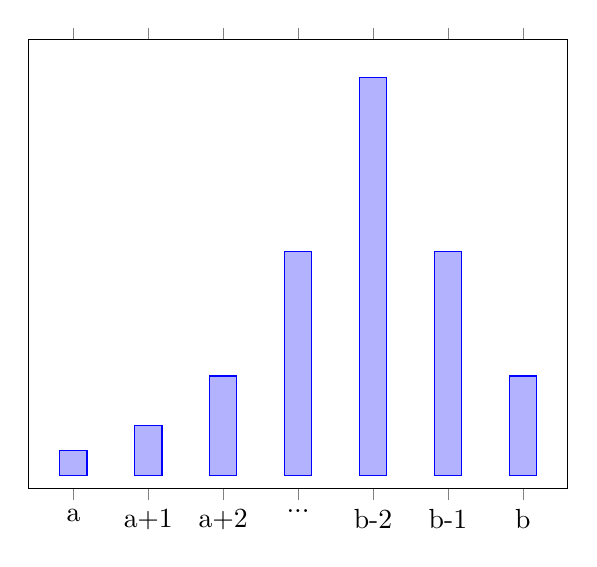
\begin{tikzpicture}
        \begin{axis}[
                ybar, 
                ytick=\empty,
                symbolic x coords={a,a+1,a+2,...,b-2,b-1,b},
            ]
            \addplot plot coordinates
                {(a,1) (a+1,2) (a+2,4) (...,9) (b-2,16) (b-1,9) (b,4)};
        \end{axis}
    \end{tikzpicture}
    \caption{Definition einer diskreten Verteilung}
\end{figure}

Sei der Wertebereich definiert durch die Werte $a,a+1,a+2,\dots,b-2,b-1,b$ im Intervall $[a,b]$, wobei $a,b \in\mathbb{N}_0$, $x_0 \le x_n$, dann werden genau $b-a+1$ Klicks benötigt, wenn alle Säulen gesetzt werden sollen. Der Aufwand könnte erheblich reduziert werden, indem im Optimalfall mit einem einzigen haltenden Klick und einer Bewegung des Zeigers alle Säulen gesetzt werden.

Ein Problem bei dieser Funktion ist, dass oft nicht alle Säulen auf die Zeigerposition gesetzt werden, weil das mouseover-Event nicht oft genug ausgelöst wird. Dies wird durch mehrere Faktoren negativ beeinflusst:
\begin{itemize}
    \item Niedrige Skalierung des Diagramms
    \item Hohe Zeigergeschwindgkeit in horizontaler Richtung
    \item Großes Intervall $[a,b]$
 \end{itemize}

Um diesem Effekt entgegenzuwirken, kann eine Schätzung der Mausbewegung mithilfe einer linearen Interpolation vorgenommen werden. Dazu muss bei jedem Handleraufruf für das mouseDown-Event die aktuelle Position des Zeigers gespeichert werden. Der Handler für das mouseMove-Event hat dann immer die Koordinaten für die letzte und aktuelle Position des Zeigers. Seien die beiden Punkte $A(a_x|a_y), B(b_x|b_y)$ gegeben, dann ist die lineare Interpolationsfunktion für alle diskreten Werte im Intervall $[a_x,b_x]$ definiert als $f(x)=mx+a_y-m*a_x$ mit $m=\frac{b_y-a_y}{b_x-a_x}$. Alle Säulen zwischen der letzten bekannten und der aktuellen Zeigerposition können nun gesetzt werden, sodass keine Lücken mehr beim Bearbeiten der diskreten Wahrscheinlichkeitsverteilung auftreten.

\subsubsection{Interpolation der erstellten Wahrscheinlichkeitsverteilung}

Die in der Wahrscheinlichkeitsverteilung erstellten Punkte können linear miteinander verbunden werden. Oft ist ein linearer Zusammenhang nicht realistisch genug, um eine Wahrscheinlichkeitsverteilung zu beschreiben. Um gekrümmte Verbindungen zwischen den Punkten zu erstellen, kann eine sogenannte Spline-Interpolation verwendet werden. Chart.js bietet bereits Interpolationsmöglichkeiten, die für die Visualisierung eingesetzt werden können, jedoch gibt es keine geeignete Schnittstelle, um auf die Interpolationsdaten zuzugreifen. Ein Spline-Algorithmus muss deshalb selbst implementiert werden. Die genaue Spline-Funktion wird zwingend benötigt, um die Werte zwischen den erstellten Punkte berechnen zu können. 

Es gibt eine Menge Vorgehensweise, um passende Splinefunktion zu finden. 
Kubische Splines interpolieren eine Menge von Kontrollpunkten mit Hilfe von
stückweise kubischen Polynome. Die Verwendung von Polynomen niederer Ordnung ist für die Kurvenanpassung besonders attraktiv, da sie sehr performant sind und numerischen Instabilitäten verhindern, die bei höhergradigen Kurven entstehen können. Diese Instabilitäten verursachen unpassendes Kurvenverhalten, durch die Punkte, die in einer gemeinsamen Kurve verbunden werden. Höhergradige Funktionen sind oft zu aufwändig bei der Berechnung, um sie für Interpolationszwecke einzusetzen. Das wohl überzeugendste
Argument der kubisch hermiteschen Interpolation ist ihre $C^2$-
Kontinuität, die garantiert, dass sich die Splinefunktion kontinuierlich über die erste und zweite Ableitung aller Polynomsemente hinweg fortsetzt.
Kontinuität erzwingt einen glatte Transition über die ganze Kurve hinweg \cite{Wolberg1999}.

Bezüglich der Gesaltung einer Wahrscheinlichkeitsverteilung, soll die Splinefunktion so bestimmt werden können, dass die gewünschte Wahrscheinlichkeitsverteilung am einfachsten und intuitivsten erstellt werden kann. Die kurvenartige Struktur von Splines ermöglicht es zwar realistische bzw. glatte Kurven zu erstellen, ein Problem, das sich bei den meisten Splines aber herausstellt ist ihre Tendenz zu überschwingen. 

Überschwingen ist die Bezeichnung für eine sprunghafte Änderung, wodurch die Funktion über den eigentlich angezielten Wert hinausschießt und sich erst im weiteren Verlauf dem eigentlichen Wert annähert. Leider neigen kubisch hermitesche Splines zu diesem Überschwingen, weshalb ihre Nutzung in dieser Form hier ungünstigt ist \cite{kruger:2007}.

\begin{figure}[H]
    \center
    \begin{tikzpicture}
        \begin{axis}[nodes near coords={(\coordindex)},
            xmin=0,
            xmax=3,
            ymin=0,
            ymax=10
        ]
        \addplot[
            mark=*,
            patch,mesh,
            patch type=cubic spline]
        coordinates {
            % left, right, left middle, right middle
            (0,1) 
            (3,9)
            (1,6)  
            (2,2)
        };
        \end{axis}
    \end{tikzpicture}
    \caption{Spline mit Überschwingen}\label{fig:spline}
\end{figure}

In der Abbildung \ref{fig:spline} ist ein kubisch hermitescher Spline zu erkennen, der zwischen den vier Kontrollpunkten $P_1(0,1)$, $P_2(1,6)$, $P_3(2,2)$ und $P_4(3,9)$ interpoliert. Es is deutlich zu erkennen, wie das Splinepolynom zwischen $P_1$ und $P_2$ über den y-Wert von $P_2$ überschwingt. Auch zwischen $P_3$ und $P_4$ ist ein Unterschwingen zu erkennen.

Gerade bei der Erstellung einer Wahrscheinlichkeitsverteilung ist es wichtig für bestimmte Stellen Extrema festlegen zu können. Beginnt die Wahrscheinlichkeitsverteilung an Extremstellen zu überschwingen, erschwert das Über- bzw. Unterschwingen passgenaue Wahrscheinlichkeitsverteilungen zu erstellen, wodurch das Endresultat verfälscht wird. 

Um das Über- und Unterschwingen zu verhindern muss die Monotonie-Eigenschaft der Splinefunktion garantiert werden.

\begin{figure}[H]
    \center
    \begin{tikzpicture}
        \begin{axis}[
            xmin=0,
            xmax=3,
            ymin=0,
            ymax=10]
        ]
        \addplot+[smooth] coordinates {
            (0,1) 
            (1,6)  
            (2,2)
            (3,9)
        };
        \end{axis}
    \end{tikzpicture}
    \caption{Monotone Kubische Interpolation}\label{fig:monotonespline}
\end{figure}

In der Abbildung \ref{fig:monotonespline} ist ein monotoner kubischer hermitescher Spline gezeichnet mit identischen Kontrollpunkten zu der Abbildung \ref{fig:spline}. Bei dieser Splinefunktion ist der Monotoniecharakter dadurch zu erkennen, dass sowohl das Überschwingen als auch das Unterschwingen verhindert wird, was ein intuitiveres Kurvenverhalten fördert.

Eine sehr einfache Art Punkte monoton kubisch zu interpolieren erarbeiten Fritsch und Carlson in ihrem Paper von 1980. Sie stellen notwendige und ausreichende Bedingungen für die Monotonie der Spline-Polynome auf. Der Fritsch-Carlson-Algorithmus macht eine einfache erste Schätzungen der Tangentensteigungen und übergibt dann erneut Datenpunkte, um eventuelle überschwingende Tangenten in die monotone Region zu verschieben \cite{Fritschcarlson:1980}. Es gibt andere Algorithmen wie zum Beispiel die Fritsch-Butland-Methode, der aufwändigere erste Schätzungen von Tangenten macht, sodass die Tangenten garantiert im monotonen Bereich liegen und kein zweiter Durchgang erforderlich ist \cite{Fritschbutland:1984}.

Da sich die Fritsch-Carlson-Methode vergleichsweise schnell und einfach implementieren lässt, wird die Fritsch-Carlson-Methode für die monotone kubische Interpolation verwendet.

Die Fritsch-Carlson-Methode beschreibt einen Weg interpolierende Tangentensteigungen für jeden Kontrollpunkt so zu wählen, dass alle Splinesegmente monoton bleiben. Wie bereits erwähnt benötigt die Methode zwei Durchläufe. 

Seien die Kontrollpunkte gegeben durch $P_i(x_i,y_i)$ für $1\le i \le n$.
Im ersten Durchlauf wird durch für den ersten bis zum letzten Kontrollpunkt, d.h. für $i=1,\dots,n-1$, die Steigung zum darauffolgenden Kontrollpunkt berechnet mit 
$$delta_i=\frac{y_{i+1}-y_i}{x_{i+1}-x_i}$$lpl
Die vorläufige Tangentensteigung für alle Kontrollpounkte bis auf die Randknoten, d.h. für $i=2,\dots,n-1$, ist dann bestimmt als der Median der beiden Steigunden zum vorherigen und folgenden Kontrollpunkt.
$$m_i=\frac{delta_{i-1}+delta_i}{2}$$
Wenn es ein Vorzeichenwechsel bei den Steigungen gibt, dann ist der Kontrollpunkt $P_i$ ein lokales Extremum. In diesem Fall muss die Steigung an der Stelle $x_i$ auf $0$ gesetzt werden, d.h.
$m_i=0$, wenn $delta_i\cdot delta_{i-1} < 0$.
Die Randwerte sind hierbei durch ihre einseitigen Differenzen bestimmt:
$m_1=delta_1$, $m_{n}=delta_{n-1}$.

Im zweiten Durchlauf werden die Tangentensteigungen hinreichend geprüft und korrigiert. Zunächst werden alle Sattelbereiche gefunden und die Steigungen auf $0$ gesetzt. Ein Sattelbereich ist bei einer Funktion dann vorhanden, wenn zwei sukzessive Punkte $P_i$, $P_{i+1}$ den gleichen y-Wert haben $y_i=y_{i+1}$ für $i=1,\dots,n-1$. Da aber bereits die Sekantensteigungen berechnet worden sind, kann auch überprüft werden, ob die Sekantensteigung gleich $0$ ist, d.h
$m_i=m_{i+1}=0$, wenn $delta_i=0$. Für alle restlichen Steigungen, haben
Fritsch und Carlson herausgefunden, dass die Splines dann monoton sind, wenn alle Tangenten in einem bestimmten Bereich der Alpha-Beta-Ebene liegen. 
$\alpha_i =\frac{m_i}{delta_i}$, $\beta_i =\frac{m_{i+1}}{delta_i}$
Eine robuste Wahl ist es, Alpha und Beta in einen Kreis mit Radius 3 zu setzen.
$m_i=\tau_i\alpha_i delta_i$, $m_{i+1}=\tau_i\beta_i delta_i$ mit $\tau_i=\frac{3}{\sqrt{\alpha_i^2+\beta_i^2}}$, wenn $\alpha^2+\beta^2>9$. \cite{Fritschcarlson:1980}

In dem folgenden Listing \ref{Fritsch-Carlson} wird in vereinfachter Form beispielhaft der Fritsch-Carlson-Algorithmus in JavaScript implementiert.
\begin{lstlisting}[caption=Fritsch-Carlson Methode,label=Fritsch-Carlson]
    fritschCarlson(xs, ys) {
        const delta = [];
        const ms = [];
        const n = xs.length;
        for (let i = 0; i < n - 1; i++) {
            delta[i] = (ys[i + 1] - ys[i]) / (xs[i + 1] - xs[i]);
            if (i == 0) {
                continue;
            }
            if (delta[i] * delta[i - 1] < 0) {
                ms[i] = 0;
            } else {
                ms[i] = (delta[i - 1] + delta[i]) / 2;
            }
        }
        ms[0] = delta[0];
        ms[n - 1] = delta[n - 2];
        for (let i = 0; i < n - 1; i++) {
            if (delta[i] === 0) {
                ms[i] = 0;
                ms[i + 1] = 0;
            } else {
                const alpha = ms[i] / delta[i];
                const beta = ms[i + 1] / delta[i];
                const dist = Math.pow(alpha, 2) + Math.pow(beta, 2);
                const tau = 3 / Math.sqrt(dist);
                if (dist > 9) {
                    ms[i] = tau * alpha * delta[i];
                    ms[i + 1] = tau * beta * delta[i];
                }
            }
        }
        return ms;
    }
\end{lstlisting}

Zur Interpolation der Splinefunktion wird das kubische hermitesche Interpolationspolynom benötigt. Zunächst muss dafür im ersten Schritt das zu dem x-Wert passende Polynom gesucht werden. Da die berechneten Steigungen aus dem Fritsch-Carlson-Algorithmus in sortierter Reihenfolge vorliegen, kann eine binäre Suche verwendet werden.
Ist das richtige Polynom p gefunden, ist die Interpolation an der Stelle t durch das Polynom
$$p_i(t)=(2t^3-3t^2+1)p_i+(t^3-2t^2+t)m_i+(-2t^3+3t^2)p_{i+1}+(t^3-t^2)m_{i+1}$$
definiert \cite{Pat:2009}.

\subsubsection{Bestimmung der inversen kummulativen Wahrscheinlichkeitsverteilung}

Ist eine Splinefunktion für die Wahrscheinlichkeitsverteilung erstellt, besteht der letzte Schritt darin, die inverse kummulative Wahrscheinlichkeitsverteilung zu bestimmen. Da es, wenn überhaupt, nur mit großem Aufwand möglich ist die inverse kummulative Wahrscheinlichkeitsverteilung unmittelbar rechnerisch zu berechnen, wird stattdessen eine Approximation durchgeführt. 

Im ersten Schritt wird die Splinefunktion schrittweise interpoliert, sodass eine Menge von Punkten die Splinefunktion beschreiben. Die erhaltenen Punkte beschreiben die Dichtefunktion oder englisch PDF (probability density function). 

\begin{figure}[H]
    \centering
    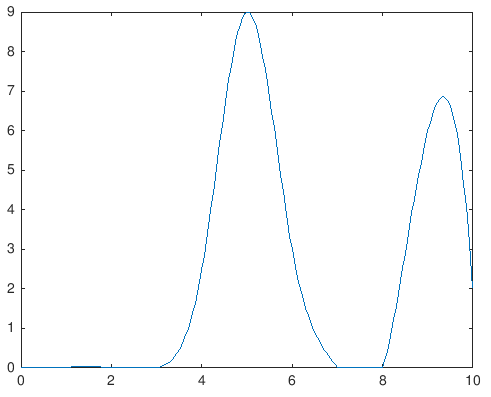
\includegraphics[height=.35\textwidth]{spline_pdf.png}
    \caption{Spline PDF}\label{fig:pdf}
\end{figure}

Die Abbildung \ref{fig:pdf} zeigt eine beispielhafte Dichtefunktion. Für $x=5$ und $x=9$ soll die Wahrscheinlichkeit am größten sein zufällig generiert zu werden. In den Intervallen $[0;2.5]$ und $[6.5,8]$ ist die Dichtefunktion gleich $0$, wodurch Werte innterhalb dieser Intervalle nicht generiert werden können.

Die Dichtefunktion kann nun integriert werden, indem  kummulativ der Flächeninhalt für jeden interpolierten Datenpunkt bestimmt wird. Das Ergebnis ist die Wahrscheinlichkeitsfunktion oder englisch CDF (kumulative distribution function) \cite{denker:2008}.

\begin{figure}[H]
    \centering
    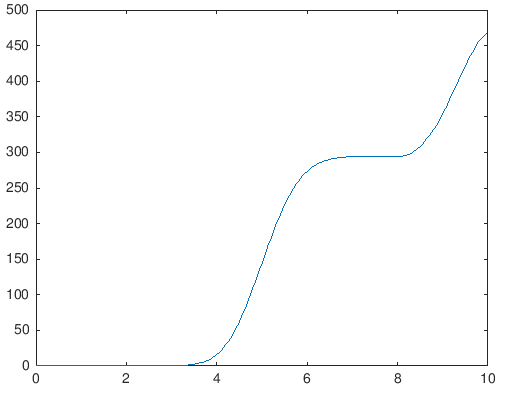
\includegraphics[height=.35\textwidth]{spline_cdf.png}
    \caption{Spline CDF}\label{fig:cdf}
\end{figure}

Eigentlich sollte die eingeschlossene Fläche der Dichtefunktion $sum(pdf)$ gleich $1$ sein. Dies stellt jedoch kein Problem dar, da die $cdf$ auf $1$ normiert werden kann, indem jeder y-Wert der $cdf$ durch $sum(pdf)$ geteilt wird.

\begin{figure}[H]
    \centering
    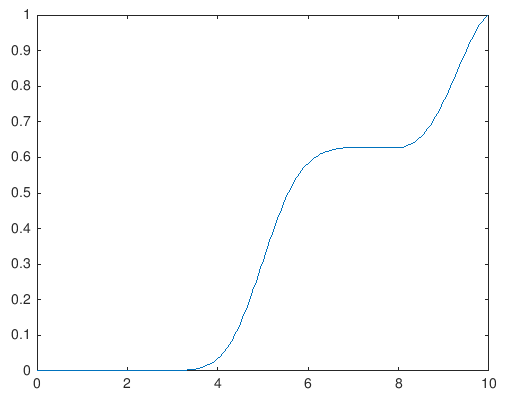
\includegraphics[height=.35\textwidth]{spline_cdf_norm.png}
    \caption{Spline CDF Normiert}\label{fig:cdfnorm}
\end{figure}

Das Ergebnis der Normierung wird in der Abbildung \ref{fig:cdfnorm} gezeigt.
An dieser Stelle wird die Inversionsmethode verwendet, um eine $U(0,1)$-verteilte Zufallsvariable auf eine vorgegebene Wahrscheinlichkeitsfunktion $F$ abzubilden \cite{Inversionsmethode}. Dafür wird ein gleichverteilter Zufallswert auf der vertikalen Achse generiert und der zugehörige Wert auf der Wahrscheinlichkeitsfunktion gesucht. Der erhaltene Zufallswert unterliegt nun der vorgegebenen Wahrscheinlichkeitsverteilung.

\begin{figure}[H]
    \centering
    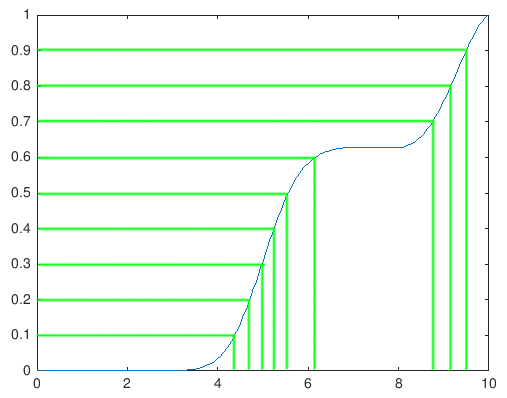
\includegraphics[height=.35\textwidth]{spline_cdf_norm_ex.png}
    \caption{Spline CDF Normiert}\label{fig:cdfnormex}
\end{figure}

Anschaulich kann die beschriebene Methode in der Abbildung \ref{fig:cdfnormex} betrachtet werden. Durch die grünen Linien wird verdeutlicht, dass ein relativ großer Bereich auf der vetikalen Achse von ca. $0.1$ bis $0.6$ auf einen vergleichsweise kleineren Bereich auf der hoizontalen Achse von ca. $4$ bis $6$ abgebildet wird. Die Autrittswahrscheinlichkeit ist für die Werte $5$ und $9$ am größten.

\section{Web Worker}
JavaScript ist im Browser single-threaded. Das bedeutet, dass die Webseite \enquote{einfriert}, wenn eine Berechnung lange benötigt. Es kann also keine Interaktion mit der Seite mehr vorgenommen werden \cite{googledev:webworkers}. Solche Interaktionen sind beispielsweise das Klicken auf Buttons oder das Scrollen der Seite.

Für diese Arbeit muss jedoch eine große Anzahl von Datensätzen generiert werden. Dies soll möglichst schnell geschehen; gleichzeitig soll die Applikation trotzdem bedienbar bleiben und einen Fortschrittsbalken anzeigen.

Um diese Anforderungen umzusetzen, werden sogenannte \textit{Web Worker} verwendet. Web Worker werden in separaten Hintegrundthreads ausgeführt und blockieren dadurch nicht den Hauptthread \cite{mdn:webworkers}. Da JavaScript nicht multithreading-fähig ist, besitzen der Hauptthread und die Web Worker keinen geteilten Adressraum. Es können also keine Objektreferenzen aus dem Hauptthread im Web Worker oder andersherum verwendet werden \cite{mdn:webworkers}.

\subsection{Übertragen von Daten zwischen Workern und Hauptthread}

Die Kommunikation zwischen Hauptthread und Web Workern funktioniert über Nachrichten. Jeder Nachricht können Daten beigefügt werden. Weil keine Referenzen verwendet werden können, werden die Daten kopiert \cite{mdn:webworkers}.

Um komplexe Datentypen zwischen Workern und dem Hauptthread zu übertragen, gibt es mehrere Möglichkeiten:
\begin{itemize}
    \item \textbf{Serialisierung über JSON}: Über die Standardfunktionen \texttt{JSON.stringify()} und \texttt{JSON.parse()} können komplexe Datentypen serialisiert beziehungsweise deserialisiert werden. So kann beispielsweise ein Objekt im Worker serialisiert werden, der entstandene String über \texttt{postMessage()} an den Hauptthread übertragen werden und das Objekt dort deserialisiert werden. Mit dieser Methode können keine zyklischen Objekte (also Objekte, die eine Referenz auf sich selber enthalten) serialisiert werden \cite{mdn:json_stringify}; dies stellt aber im Kontext dieser Arbeit kein Problem dar.
    \item \textbf{Structured Cloning}: Für die Übergabe von Objekten von und zu Workern wurde der Structured Cloning Algorithmus entwickelt. Dieser klont die Objekte und unterstützt dabei auch zyklische Referenzen \cite{mdn:structured_cloning}.
    \item \textbf{Transferables}: Transferable Objects sind Objekte, die zwischen JavaScript-Kon\-texten transferiert werden können. Dabei werden die Objekte nicht kopiert. Stattdessen wird die Referenz auf das Objekt im Ursprungskontext zerstört und im Zielkontext angelegt \cite{googledev:transferables}. Dadurch wird weiterhin eine Threadsicherheit gewährleistet.
\end{itemize}

Auch wenn Transferables in der Theorie die schnellste Art sein sollten, Daten auszutauschen, zeigt sich in der Praxis, dass es stark auf die Art der Daten ankommt, welche Methode die schnellste ist \cite{transferables1, transferables2, transferables3}.

Die generierten Daten werden in der entwickelten Applikation in einem Array von Objekten gespeichert. Jedes Objekt stellt dabei einen einzelnen Datensatz dar, wobei die Schlüssel innerhalb des Objekts die Spaltennamen abbilden.

Arrays sind in JavaScript nicht transferable. Das bedeutet, dass das generierte Array zuerst in einen binären ArrayBuffer überführt werden müsste. Dieser Vorgang macht den Geschwindigkeitsvorteil von Transferables wieder zunichte, so dass entschieden wurde, die generierten Daten letztendlich über den Structured Clone Algorithm zu übertragen.

\subsection{Ablauf der Datengenerierung}

Die Datengenerierung läuft nach folgendem Muster ab:

\begin{enumerate}
    \item Es werden so viele Web Worker gestartet, wie in den Einstellungen festgelegt wurden (standardmäßig 4)
    \item Die Anzahl der zu generierenden Daten wird auf die verschiedenen Worker aufgeteilt. Jeder Worker erhält eine Nachricht mit folgendem Inhalt:
    \begin{itemize}
        \item Modell (Graph), gespeichert von BaklavaJS
        \item Index des ersten zu berechnenden Datensatzes
        \item Index des letzten zu berechnenden Datensatzes
    \end{itemize}
    \item Jeder Worker hat eine eigene Instanz eines BaklavaJS-Editors mit dem Engine-Plugin. Das in der Nachricht enthaltene Modell wird geladen
    \item In einer Schleife werden die Datensätze zwischen Anfangs- und Endindex generiert. Wenn mehr als 10.000 Datensätze generiert werden, werden die Zwischenergebnisse alle 10.000 Datensätze über eine Nachricht an den Hauptthread geschickt. Dadurch wird verhindert, dass der Hauptthread (und damit die gesamte Applikation) einfriert, wenn ein Worker am Ende beispielsweise 500.000 Datensätze an den Hauptthread schickt, welcher die Daten verarbeiten muss.
\end{enumerate}

\section{Dateispeicherung}

Idealerweise sollten die Daten parallel zur Generierung bereits in die Ausgabedatei geschrieben werden. Damit kann die Arbeitsspeicherauslastung gering gehalten werden, was besonders auf Geräten mit kleinem Arbeitsspeicher, wie zum Beispiel günstigen Laptops oder bei Mobilgeräten wichtig ist. Allerdings ist mit JavaScript in Browsern aus Sicherheitsgründen kein direkter Zugriff auf das Dateisystem möglich. Dadurch ist es schwierig, die Datei sequentiell zu schreiben.

Die Bibliothek \textit{StreamSaver.js} versucht, dieses Problem zu lösen \cite{streamsaver}. Dafür benutzt sie einen \textit{Service Worker}. Service Worker haben die Möglichkeit, Webseiten offline verfügbar zu machen, indem sie HTTP-Anfragen abfangen \cite{mdn:serviceworker}. StreamSaver.js nutzt diese Möglichkeit, um einen Download-Stream zu öffnen. Dieser wird vom Browser wie bei einem normalen Dateidownload sequentiell in das Dateisystem geschrieben.

\begin{figure}[H]
    \centering
    \begin{sequencediagram}
        \newthread{mt}{Hauptthread}
        \newinst[1]{sw}{Service Worker}
        \newinst[1]{b}{Browser}

        \begin{call}{mt}{1. Get URL}{sw}{2. URL}\end{call}

        \begin{messcall}{mt}{3. Download URL}{b}
            \begin{call}{b}{4. Fetch URL}{sw}{5. Stream}\end{call}
        \end{messcall}

        \begin{sdblock}{Loop}{}
            \begin{messcall}{mt}{6. Write Data}{sw}
                \begin{messcall}{sw}{
                    \shortstack{7. Write Data \\ to Stream}}{b}\end{messcall}
            \end{messcall}
        \end{sdblock}

        \begin{messcall}{mt}{8. End}{sw}
            \begin{messcall}{sw}{9. Close Stream}{b}\end{messcall}
        \end{messcall}

    \end{sequencediagram}
    \caption{UML-Sequenzdiagramm Download mit StreamSaver.js}
    \label{fig:streamsaverflow}
\end{figure}

\begin{enumerate}
    \item Der Hauptthread initiiert den Vorgang indem er eine Nachricht an den Service Worker schickt
    \item Der Service Worker generiert eine Download-URL und schickt dem Hauptthread eine Nachricht zurück, die die Download-URL und einen speziellen Kommunikationskanal enthält, über den der Hauptthread Daten für diese URL an den Service Worker schicken kann
    \item Der Hauptthread weist den Browser an, einen Download auf die erhaltene URL zu starten
    \item Der Browser schickt eine HTTP-Anfrage an die URL. Der Service Worker erkennt, dass die URL eine von ihm generierte URL ist und fängt die Anfrage ab
    \item Der Service Worker öffnet einen Stream, um dem Browser die Antwort zu schicken
    \item Der Hauptthread schickt über den erhaltenen Kommunikationskanal Daten an den Service Worker
    \item Der Service Worker erhält diese Daten und schreibt sie in den Stream, welcher in Schritt 5 geöffnet wurde
    \item Der Hauptthread beendet die Kommunikation, indem er den speziellen Kommunikationskanal schließt
    \item Der Service Worker erkennt, dass der Kommunikationskanal geschlossen wurde und schließt den Download-Stream. Damit erkennt der Browser, dass der Download abgeschlossen ist und markiert dies entsprechend in der grafischen Benutzeroberfläche des Browsers
\end{enumerate}

Dieser Ansatz hätte es erlaubt, die generierten Daten schon parallel zur Generierung in eine Datei zu schreiben und damit die Arbeitsspeicherauslastung gering zu halten. Leider konnte die Bibliothek in dieser Arbeit nicht zum Laufen gebracht werden; auch eine eigene Umsetzung schlug fehl. Aus diesem Grund werden in der finalen Implementierung dieser Arbeit erst alle Daten in den Arbeitsspeicher geladen und anschließend ein Download auf die Gesamtdatenmenge gestartet. Dies ist mit einfachen JavaScript-Funktionen umsetzbar.